\documentclass{beamer}
\usetheme{Malmoe}
\usecolortheme{beaver}
\useoutertheme{miniframes}
\useinnertheme{circles}

% Required packages
\usepackage{verbatim}
\usepackage{xcolor}
\usepackage{graphicx}
\usepackage{listings}
\usepackage{textcomp}

% Include custom theme and color definitions
\usepackage{RCRDtheme}

% Configure spacing and presentation settings
\setlength{\parskip}{0.5em}
\setbeamertemplate{navigation symbols}{}  % Remove navigation symbols
\setbeamertemplate{footline}[frame number]  % Add frame numbers
\setbeamertemplate{frametitle continuation}[from second]

% Title page information
% Presentation structure
\AtBeginSection[]
{
  \begin{frame}
    \frametitle{Contents}
    \tableofcontents[currentsection]
  \end{frame}
}

\title{Software Development Process}
\subtitle{Or how the He LLMs do I do this?}
\author{Luke Herbert}
\date{\today}

\begin{document}

\begin{frame}[plain]
    \begin{columns}[T]
        \begin{column}{0.6\textwidth}
            \titlepage
        \end{column}
        \begin{column}{0.4\textwidth}
            \vspace{1cm}
            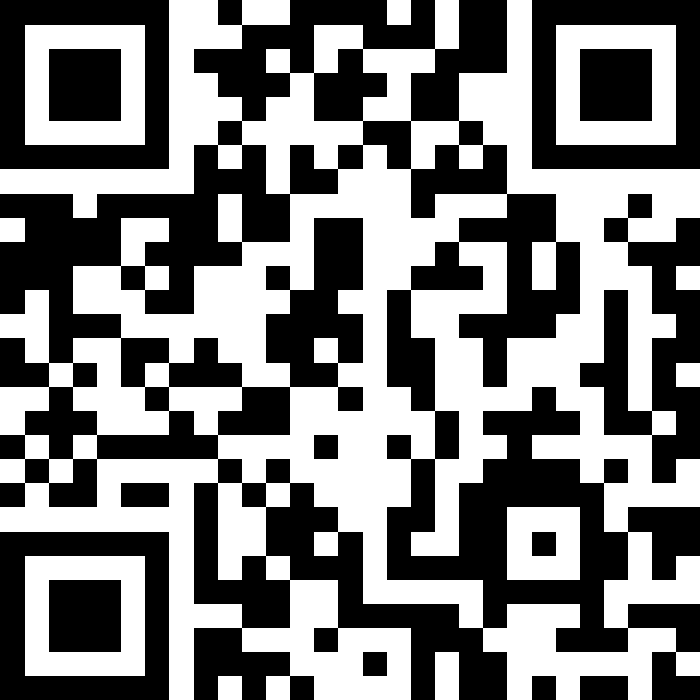
\includegraphics[width=\textwidth]{QR Code for LLM use.png}
        \end{column}
    \end{columns}
\end{frame}

\begin{frame}
    \frametitle{Presentation Overview}
    \tableofcontents
\end{frame}

\begin{frame}
    \frametitle{The Issue with LLMs}
    \begin{center}
        I would like a three legged stool or frame so that I can show that each of the three legs of my process - LLM, meta documents and testing framework - are equally important.
        \pause
        \vspace{0.5cm}
        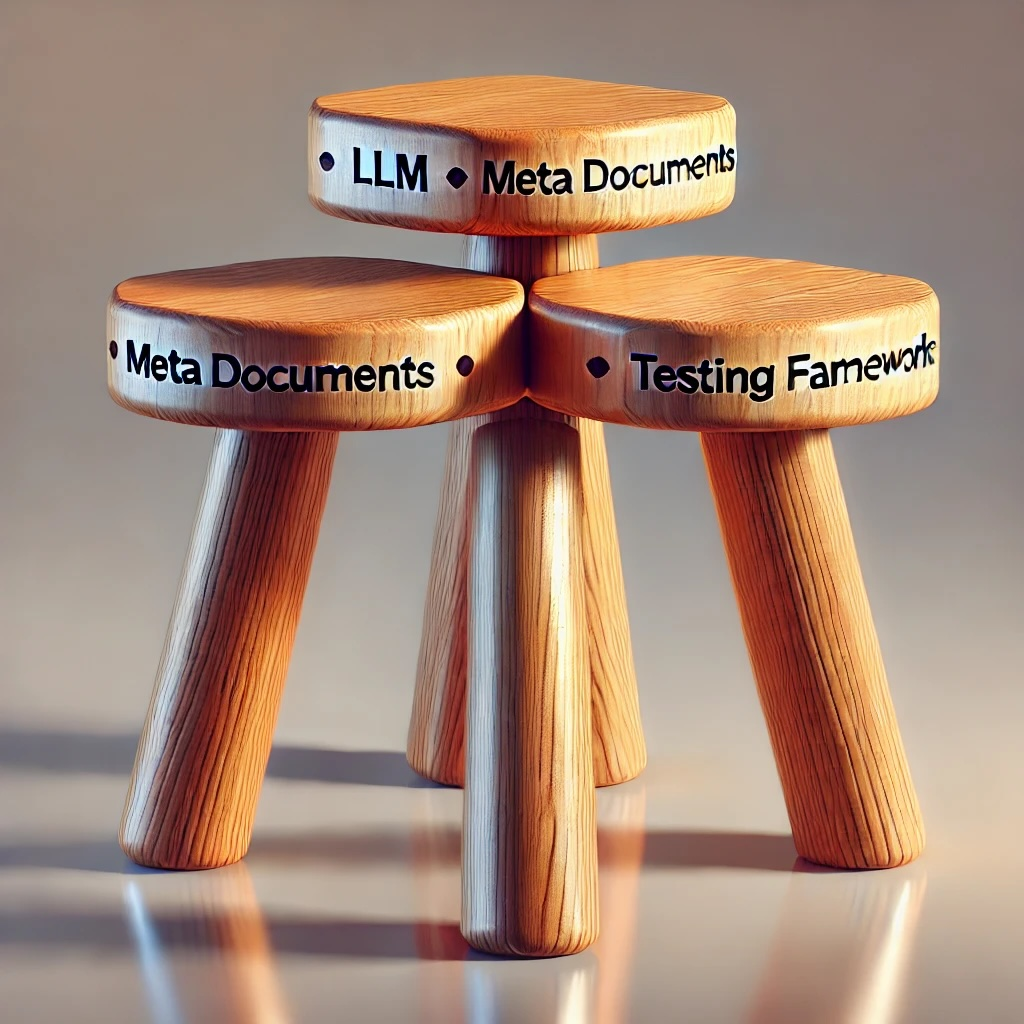
\includegraphics[height=0.6\textheight]{stool.jpg}
    \end{center}
\end{frame}

\section{Development Tools Overview}
\begin{frame}
    \frametitle{Integrated Development Approach}
    \begin{block}{Three Parallel Tools}
        \begin{enumerate}
            \item Meta Documents \pause
            \item LLM Integration \pause
            \item Testing Framework and Continuous Testing \pause
        \end{enumerate}
    \end{block}
\end{frame}

\section{Meta Documents}
\begin{frame}
    \frametitle{Meta Documents Role}
    \begin{alertblock}{Living Documentation}
        \begin{itemize}
            \item Initial project scoping and design
            \item Document ongoing issues and challenges
            \item Record development ideas and iterations
            \item Track tried and abandoned approaches
            \item Serve as documentation when complete
        \end{itemize}
    \end{alertblock}
\end{frame}

\section{LLM Integration}
\begin{frame}
    \frametitle{LLM Usage}
    \begin{block}{Intelligent Assistant}
        \begin{itemize}
            \item Interprets meta documents for context
            \item Uses design guidelines for implementation
            \item References history of approaches
            \item Follows specific development instructions
        \end{itemize}
    \end{block}
\end{frame}

\begin{frame}
    \frametitle{Advantages of using meta documents and LLM}
    \begin{exampleblock}{Break Revision Cycles}
        \begin{itemize}
            \item Sometimes the  LLM will go round in circles!
            \item Provides alternative approaches
            \item Use meta documents to steer the process
            \item Use the LLM to update the meta files
        \end{itemize}
    \end{exampleblock}
\end{frame}

\section{Development Tools}
\begin{frame}
    \frametitle{Pre-commit Configuration}
    \begin{block}{Automated Quality Checks}
        \begin{itemize}
            \item Pre-commit hooks run before each commit
            \item Enforces code quality standards
            \item Runs automated tests
            \item Checks formatting and linting
        \end{itemize}
    \end{block}
\end{frame}

\begin{frame}
    \frametitle{How Pre-commit Hooks Work}
    \begin{block}{Workflow}
        \begin{enumerate}
            \item Developer stages changes with git add
            \item Pre-commit runs configured hooks
            \item Each hook checks specific aspects:
                \begin{itemize}
                    \item Code formatting
                    \item Linting rules
                    \item Test execution
                \end{itemize}
            \item Commit blocked if any hook fails
            \item Developer fixes issues and tries again
        \end{enumerate}
    \end{block}
\end{frame}

\begin{frame}
    \frametitle{Benefits of Pre-commit Hooks}
    \begin{alertblock}{Key Advantages}
        \begin{itemize}
            \item Catches issues before they enter the codebase
            \item Ensures consistent code style across team
            \item Automates repetitive quality checks
            \item Reduces code review overhead
            \item Prevents broken tests from being committed
        \end{itemize}
    \end{alertblock}
\end{frame}

\begin{frame}[fragile]
    \frametitle{Pre-commit Configuration Example}
    \begin{verbatim}
repos:
-   repo: https://github.com/pre-commit/pre-commit-hooks
    rev: v4.4.0
    hooks:
    -   id: trailing-whitespace
    -   id: end-of-file-fixer
    -   id: check-yaml
    -   id: check-added-large-files

-   repo: https://github.com/psf/black
    rev: 23.3.0
    hooks:
    -   id: black

-   repo: local
    hooks:
    -   id: jest-tests
        name: Run Jest Tests
        entry: npm test
        language: system
        types: [javascript]
        pass_filenames: false
    \end{verbatim}
\end{frame}

\section{Testing Framework}
\begin{frame}
    \frametitle{Testing Approach}
    \begin{block}{Flexible Testing Strategy}
        \begin{itemize}
            \item Initial minimal working application tests
            \item Parallel development with main code
            \item Focus on problem areas
            \item Regular updates to match running code
        \end{itemize}
    \end{block}
\end{frame}

\begin{frame}
    \frametitle{Test-Driven Development}
    \begin{alertblock}{TDD Cycle}
        \begin{enumerate}
            \item Write failing test first
            \item Implement minimal code to pass test
            \item Refactor while keeping tests green
            \item Repeat for next feature
        \end{enumerate}
    \end{alertblock}
    
    \begin{block}{Benefits}
        \begin{itemize}
            \item Ensures code is testable by design
            \item Prevents over-engineering
            \item Documents expected behavior
            \item Catches regressions early
        \end{itemize}
    \end{block}
\end{frame}

\begin{frame}
    \frametitle{Test Organization}
    \begin{block}{Directory Structure}
        \begin{itemize}
            \item Tests mirror source code structure
            \item Component tests in \_\_tests\_\_ directories
            \item Shared test utilities and helpers
            \item Clear separation of concerns
        \end{itemize}
    \end{block}
    
    \begin{alertblock}{Test Categories}
        \begin{itemize}
            \item Unit tests for individual components
            \item Integration tests for component interactions
            \item End-to-end tests for complete workflows
            \item Performance and accessibility tests
        \end{itemize}
    \end{alertblock}
\end{frame}

\begin{frame}
    \frametitle{Test Maintenance}
    \begin{block}{Continuous Improvement}
        \begin{itemize}
            \item Regular test suite review and updates
            \item Refactor tests as code evolves
            \item Monitor test coverage and quality
            \item Document test patterns and practices
        \end{itemize}
    \end{block}
    
    \begin{alertblock}{Common Challenges}
        \begin{itemize}
            \item Keeping tests up to date with code changes
            \item Managing test data and dependencies
            \item Balancing test coverage and maintenance
            \item Handling flaky or unreliable tests
        \end{itemize}
    \end{alertblock}
\end{frame}


\end{document}
